\documentclass{article}
\usepackage{amsmath}
\usepackage{graphicx}
\usepackage[utf8]{inputenc}
\usepackage{filecontents}

\begin{filecontents}{sutton-barton-rl.bib}
@book{10.5555/3312046,
author = {Sutton, Richard S. and Barto, Andrew G.},
title = {Reinforcement Learning: An Introduction},
year = {2018},
isbn = {0262039249},
publisher = {A Bradford Book},
address = {Cambridge, MA, USA},
abstract = {The significantly expanded and updated new edition of a widely used text on reinforcement learning, one of the most active research areas in artificial intelligence. Reinforcement learning, one of the most active research areas in artificial intelligence, is a computational approach to learning whereby an agent tries to maximize the total amount of reward it receives while interacting with a complex, uncertain environment. In Reinforcement Learning, Richard Sutton and Andrew Barto provide a clear and simple account of the field's key ideas and algorithms. This second edition has been significantly expanded and updated, presenting new topics and updating coverage of other topics. Like the first edition, this second edition focuses on core online learning algorithms, with the more mathematical material set off in shaded boxes. Part I covers as much of reinforcement learning as possible without going beyond the tabular case for which exact solutions can be found. Many algorithms presented in this part are new to the second edition, including UCB, Expected Sarsa, and Double Learning. Part II extends these ideas to function approximation, with new sections on such topics as artificial neural networks and the Fourier basis, and offers expanded treatment of off-policy learning and policy-gradient methods. Part III has new chapters on reinforcement learning's relationships to psychology and neuroscience, as well as an updated case-studies chapter including AlphaGo and AlphaGo Zero, Atari game playing, and IBM Watson's wagering strategy. The final chapter discusses the future societal impacts of reinforcement learning.}
}
\end{filecontents}

\bibliographystyle{plain}

\title{COMP 138 RL: Racetrack Problem}
\author{Tung Pham}

\usepackage{natbib}
\usepackage{graphicx}

\begin{document}

\maketitle

\section{Introduction}
For the gamers that love speed, everyone would have heard of the name Need for
Speed, a game developed by EA. It used to be my childhood favorite back in the 2000s. On the old
machine with Window XP, I used to enjoy this game to the fullest. I've played
the Need for Speed: Pursuit, which is the more recent version of the game. 

However, I've
always wondering how to efficiently taking a turn as I was always
get passed by or get throw off track when it comes to these portion of the track
is extremely difficult and you can easily get slowed down and lose the match. This prone me to thinking,
with the materials I learned in CS138, can I essentially applies any of the techniques 
I learn so far into figure out the most efficient way to take a turn?

In this experiment, I'll use 2 approaches to figure this out, an Off-policy
Monte Carlo Control and Double Q-Learning Temporal Difference method. Both
methods allow the driver to learn from the experience of the environment by
having a learning strategy that will be improve over the training courses.
Eventually, the learning approaches, or policy denoted $\pi$, can leads to the agent figure out the
optimal way to turn and able to achieve the highest score ($R_t$). After each attempt,
episode, the driver will have a better understanding of the environment using
the learning approach and therefore getting better score result. 

\section{Problem}
To make the problem a little less complex, I'll use a 2D matrix as my
representation of the racetrack. We'll also ignore most of the physics
mechanism as listed here:
\begin{itemize}
  \item Centripetal force
  \item Inertia
  \item We won't be using any metrics like kilometer but instead will be relying
    on the matrix unit.
  \item We'll also not using seconds as the time step but instead a time step
    is relying on the clock speed of the computer that used to simulate.
  \item No air friction.
\end{itemize}

We'll also assume some idealistic scenario:
\begin{itemize}
  \item The racetrack doesn't have any bumps and is a smooth curve
  \item Acceleration happens in integer values
  \item The maximum velocity the driver can get is 5 matrix unit.
  \item When the car move to the next location on the grid, it will have a
    teleportation behavior and jumping straight to the location, but if the
    location is out of bound, it will fall off.
  \item When the car falls off, it will be teleported back to a random location
    on the starting line and retrying the race.
  \item If the driver go too fast and the next location he arrive is not the
    finish line, he'll be out of bound and fall off the racing track.
\end{itemize}

At each time step, the driver can decided to hit the brake or hit the gas which
will decelerate or accelerate the car by 1 matrix unit respectively. 
To make things a little challenging to the driver, at 10\% of the time the brake and gas pedal won't work 
because of how smooth the racetrack it and cause the car to slip and no friction
was applies which cause no acceleration or deceleration can occurs.

The score of the action that the driver takes will be accumulated through out
each attempt and the average over all the attempts will be measured.

In this experiment, we'll be doing 2000 attempts on 2 different tracks using
each method. We're also conducting some initial tests that was used on 2 other
smaller size grid which can be seen in Figure 2 and Figure 3.

\begin{figure}[h!]
\centering
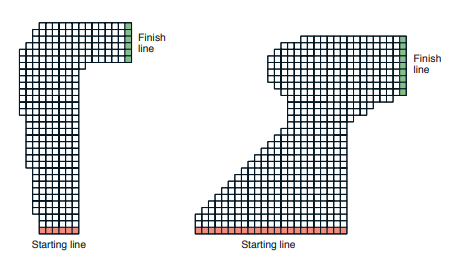
\includegraphics[scale=0.9]{./images/book-race-track.png}
\caption{The large race track that was used for experiment}
\label{fig:book-race-track}
\end{figure}

\begin{figure}[h!]
\centering
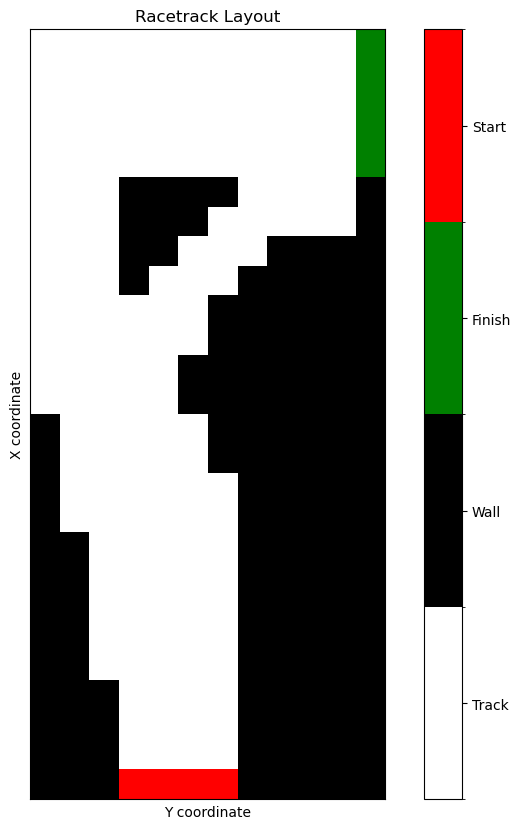
\includegraphics[scale=0.2]{./images/test_racetrack1.png}
\caption{Smaller test racetrack 1}
\label{fig:test-racetrack1}
\end{figure}

\begin{figure}[h!]
\centering
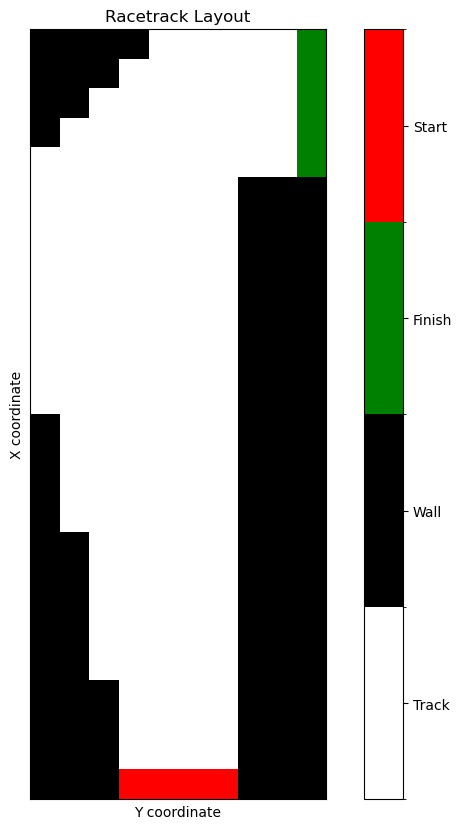
\includegraphics[scale=0.2]{./images/test_racetrack2.png}
\caption{The second smaller test racetrack}
\label{fig:test-racetrack2}
\end{figure}

\section{Methodology}
\subsection{Environment}
To represent the racetrack, we'll be using a 2D grid. However, as you'll see
later on, because the track is upside down in the code matrix, we'll have to
flip the matrix so that the environment is correctly represent that the driver
or the car is going from the bottom up.

To represent the state, since there are 4 values that is in effect in this
problem which is the position on the grid and the velocity. Since this is a
grid, we'll need the coordinate which is x value and the y value. Also for the
velocity, since we'll be moving in both x and y direction, we'll need to track
the 2 velocity as well. Our state eventually becomes a tuple of (x coordinate, y
coordinate, vx, vy).

Then at each step taken all the criterias mentioned in the problem statement
will be in effects to determine the out-of-bound and the destination. It will
also handles teleport the driver or the car back to the starting position.

\subsection{Off-policy Monte Carlo Control}
\subsubsection{Setup}
In Chapter 5.8 of Sutton and Barton, we were introduced with an off-policy Monte
Carlo Control algorithm which is described in Figure 4.

\begin{figure}[h!]
\centering
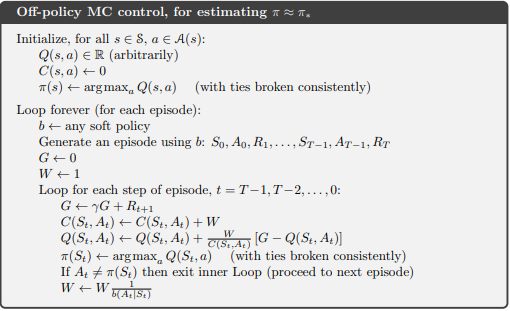
\includegraphics[scale=0.9]{./images/op-mc-algo.png}
\caption{The Off-policy Monte Carlo Control algorithm in Sutton and Barton
\cite{sutton-barton-rl}}
\label{fig:op-mc-algo}
\end{figure}

The algorithm starts out with initializing Q with arbitrarily non negative
floating valule. In our case, we're initializing Q with a uniform distribution
between 0 and 1 for all actions at state 0. This encourages the driver to
explore more possbilities in the unknown environment and fail alot. However,
with these failures, the drivers will learn and do a better job next time.

Then our target policy, $\pi(s)$, is a greedy algorithm that takes the action that yields the most value or reward. 
Which can be describe as:
\[
  \pi(s) = argmax_aQ(S_t, a)
\]

This algorithm separates the behavior policy from the policy that we want to
maximize which is the target policy and behavior policy can be any soft
algorithm. In our case, we're using $\epsilon$-soft algorithm for this policy
which is described as below:
\[
  b \leftarrow argmax_ab(a|S_t)
\]
where 
\[
  b(a|S_t) \leftarrow \left\{
\begin{array}{ll}
1-\varepsilon+\varepsilon/|A(S_t)| & \text{if } a = A^* \\
\varepsilon/|A(S_t)| & \text{if } a \neq A^*
\end{array}
\right.
\]

To choose the value of $\epsilon$, since we want the driver to exploit the current
route more but also have a little of exploration, we don't want $\epsilon$ to be
too high and therefore decided to go with $0.1$. Also, since we're adding a
little bit of a challenge where at $10\%$ chance the car slipped and all
acceleration or decelleration will not work, according to the rule of
$\epsilon-soft$, we can update the behavior policy further:

\[
  b(a|S_t) \leftarrow \left\{
\begin{array}{ll}
0.1+b(a|S_t) & \text{if } a \neq A_0  \\
0.9*b(a|S_t) & \text{if } a = A_0
\end{array}
\right.
\]

where $A_0$ indicates the action of not accelerating or decellerating in any
direction.

Since this is a Monte Carlo variant algorithm, all the updates to the policy
must occurs at the end of each episode. Therefore, we'll have to initially,
generate all the possible steps that the drive will be taking. This means that
the driver has to blindly do a first attempt and will taking $T$ steps to
complete an episode. 

At each step, the driver will take an action based on the bahavior policy and
yields a reward R for that action and we define R as follows:
\begin{itemize}
  \item The car reached the goal: 100
  \item The car hit the wall or fly out of bound of the race track: -5
  \item The car take a step: -1
\end{itemize}

\subsubsection{Testing}
To test, we're running the algorithm on a smaller track and print out the 
velocity and the route that the driver took which is illustrated in Figure 5 and
Figure 6 below. 

\begin{figure}[h!]
\centering
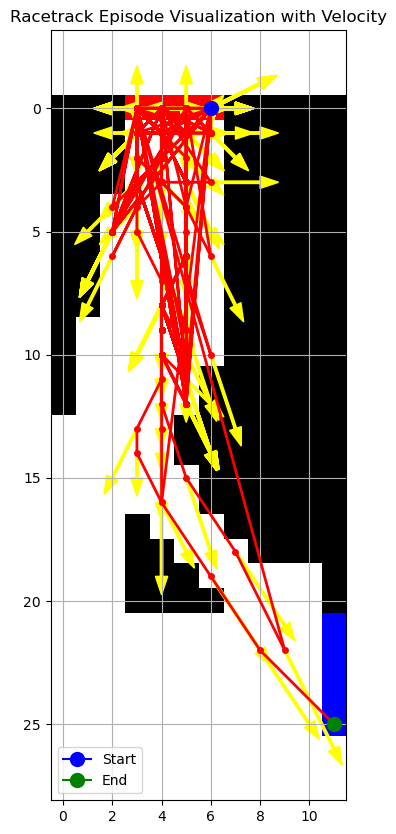
\includegraphics[scale=0.9]{./images/mc_test_racetrack1.png}
\caption{State transition of Off-policy Monte-Carlo control when run on track 1}
\label{fig:mc_test_racetrack1}
\end{figure}

\begin{figure}[h!]
\centering
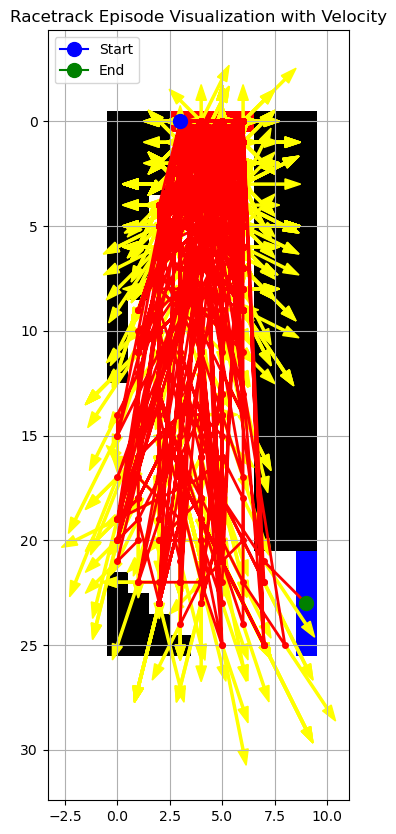
\includegraphics[scale=0.9]{./images/mc_test_racetrack2.png}
\caption{State transition of Off-policy Monte-Carlo control when run on track 2}
\label{fig:mc_test_racetrack2}
\end{figure}

Looking at the 2 figures, we can see that the step function behave correctly as
whenenever the next velocity of the action resulted in the car out of the
racetrack, we can see a straight line back to the starting point. And when the
stopping point is at the finish line, we can see that the program is successfully
end the episode.

\subsubsection{Experiment}

To do the experiment, we're then use a much larger racetrack and view the reward
change over the number of episodes. Figure 7 illustrate the average rewards over
the number of episodes as the number of episode increases on the first track and
Figure 8 is for the second track.

\begin{figure}[h!]
\centering
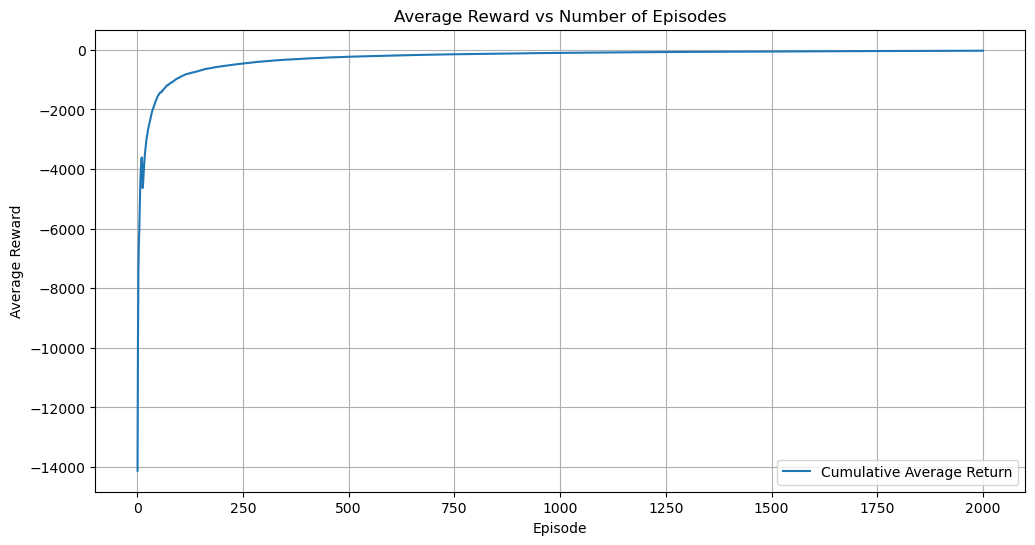
\includegraphics[scale=0.5]{./images/exp_mc_racetrack1.png}
\caption{Average reward over the episodes vs the number of episodes used for
track 1.}
\label{fig:exp_mc_racetrack1}
\end{figure}

\begin{figure}[h!]
\centering
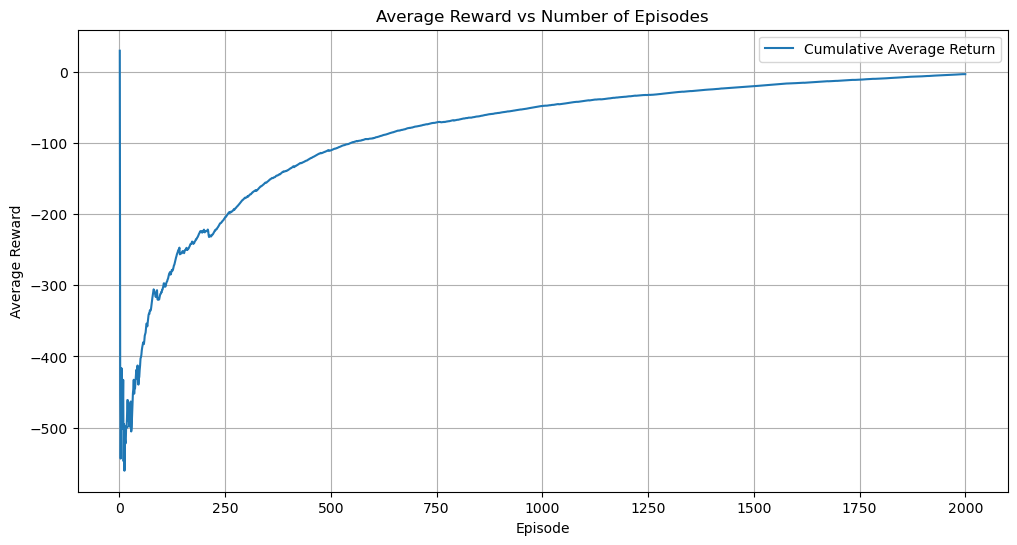
\includegraphics[scale=0.5]{./images/exp_mc_racetrack2.png}
\caption{Average reward over the episodes vs the number of episodes used for
track 2.}
\label{fig:exp_mc_racetrack2}
\end{figure}

We can see that the reward is displaying a log-like curve which gradually increase as the number of episodes
increase meaning that given enough time, the algorith can converges to the
optimal value. 

The driver at first perform extremely bad as we can see that the reward is going
all the way down to $-14000$ for track 1 and more than $-500$ for track 2.
However, since this is the first stage, the driver is exploring the unknown environment
and make a lot of mistakes. As the number of episodes increase, the reward
obtained by the driver is also increases and that cause our graph to curve up
but in the long run, we're exploiting more and less exploring, the reward began
to converges to a single value which is the optimal reward that we can get.

\subsection{Off-policy TD method with Double Q-Learning}
\subsubsection{Setup}
In Chapter 6 of Sutton and Barton, we were introduced with an off-policy TD
method algorithm with Double Q-Learning where we have 2 different Q tables that we're
keeping track with 50-50 chance to update one than the other Q table. Figure 9
illustrate this algorithm.
\begin{figure}[h!]
\centering
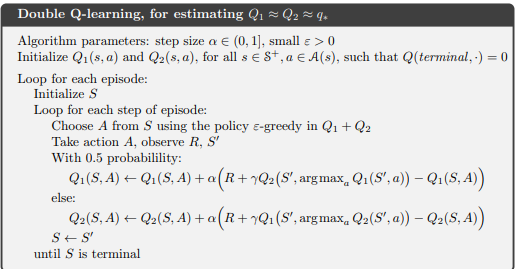
\includegraphics[scale=0.5]{./images/double-q-td-learning.png}
\caption{The Double Q-learning TD method}
\label{fig:double-q-td-learning}
\end{figure}

Since the algorithm also starts out with initializing both Qs to an arbitrary
number, we're again use uniform distribution.

To more weight on the future value, we're using a larger gamma value than
what we used in Monte Carlo which is $0.9$ but because we also want the rewards
distribution to be smoother, we're using a small value for $\alpha$.

For our greedy action selection, we're using 0.1 for our $\epsilon$ value as we
want the driver to explore options once in a while but not too often which could
steer the driver away from the optimal route.

\subsubsection{Test}
We're then testing our implementation on the smaller test set as we can see in
Figure 10 and 11.

\begin{figure}[h!]
\centering
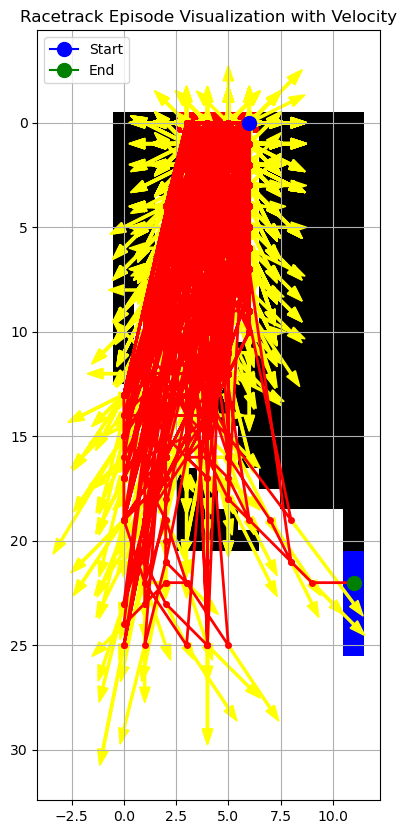
\includegraphics[scale=0.5]{./images/q-td-learning-test-track1.png}
\caption{State transition of Double Q-learning TD method runs for a single episode on a small test track 1}
\label{fig:q-td-learning-test-track1}
\end{figure}

\begin{figure}[h!]
\centering
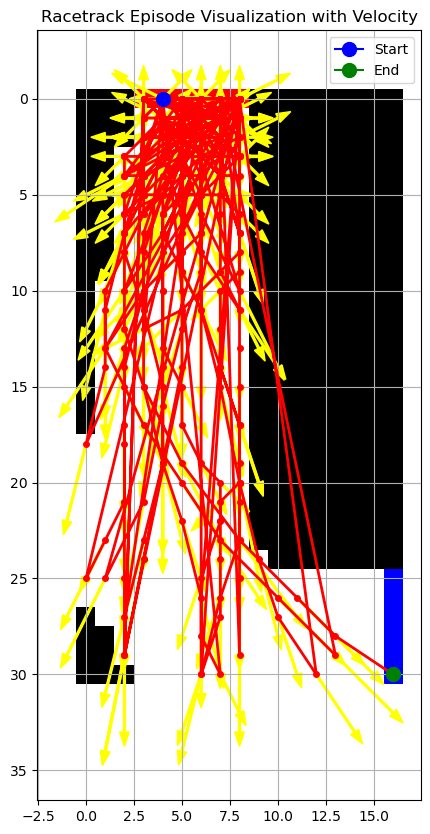
\includegraphics[scale=0.5]{./images/q-td-learning-test-track2.png}
\caption{State transition at each time step of Double Q-learning TD method runs for a single episode on a
small test track 2}
\label{fig:q-td-learning-test-track2}
\end{figure}

We can see that the driver was able to reach the destination despite the
overwhelming amount of steps taken to reach it. This is because we're running on
the initial episode and without any training, the driver doesn't learn and can't
figure out what's the best solution. Then we'll see what happens if we train the
driver with this algorithm.

\subsubsection{Experiment}
Figure 12 and Figure 13 is the plot of cummulative average reward

\begin{figure}[h!]
\centering
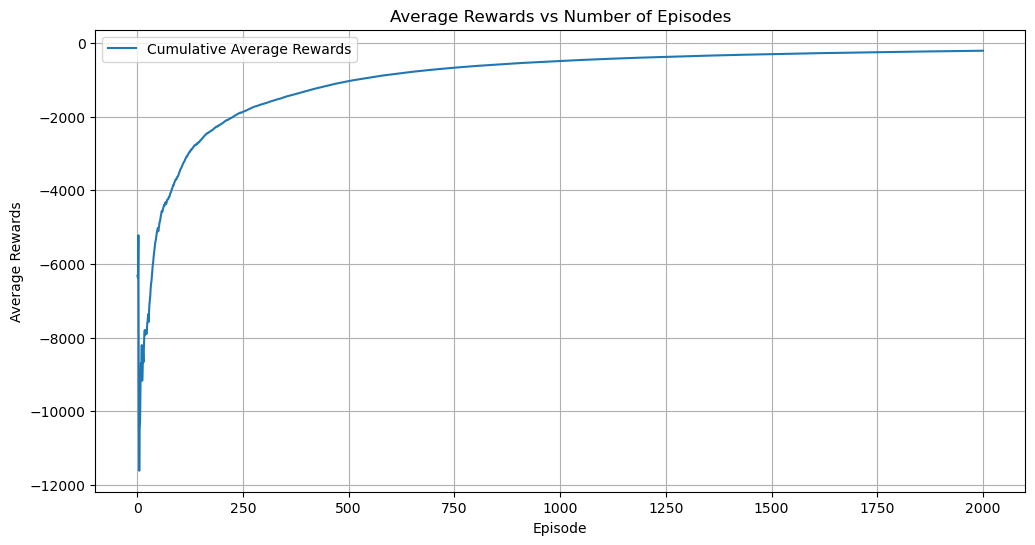
\includegraphics[scale=0.5]{./images/exp_q-td-ractrack1.png}
\caption{The Average rewards over the number of episode versus the number of
episode for Double Q-Learning TD method on track 1.}
\label{fig:exp_q-td-racetrack1}
\end{figure}
\begin{figure}[h!]
\centering
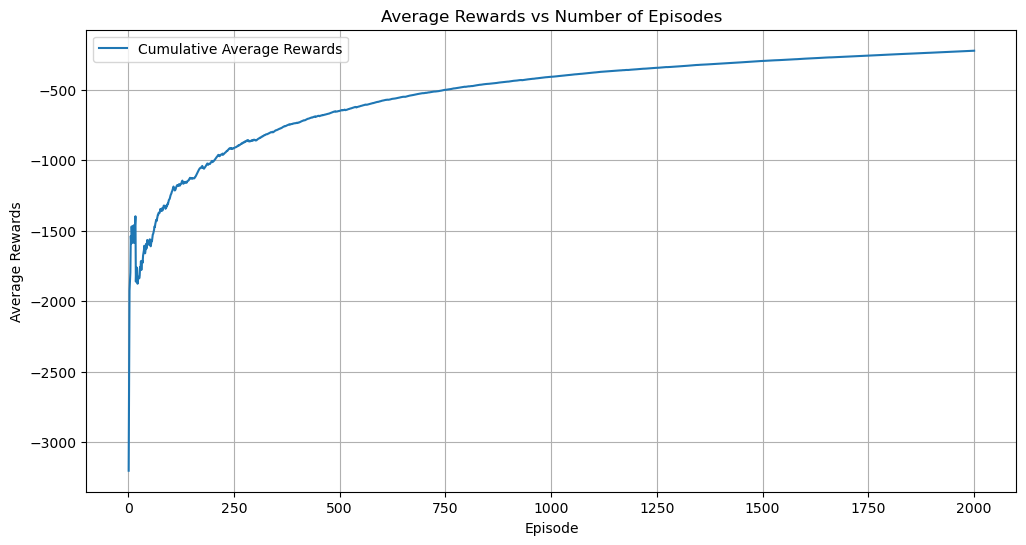
\includegraphics[scale=0.5]{./images/exp_q-td-racetrack2.png}
\caption{The Average rewards over the number of episode versus the number of
episode for Double Q-Learning TD method on track 2.}
\label{fig:exp_q-td-racetrack2}
\end{figure}

We can observe that both graphs demonstrated a bad average reward at first but
the performance increase in log-like behavior. However, the convergences point
is rather low at $-500$ which indicates that either the algorithm needs more
time to observe the convergence.

\section{Discussion}
When comparing the figures of both Monte Carlo and TD with Q-learning algorithm,
we can see that both approaches yield a desireable results. However, the
convergence point of Q-Learning is much lower than Monte Carlo indicates that
the algorithm needs more fine tuning of its parameters or more episodes in order
to achieve the same or better result. A lower convergent point also suggest that
TD approach is yielding overall less rewards than Monte-Carlo and is not
reaching the optimality as good as Monte-Carlo.

When comparing the performance of both algorithm, TD took a lot faster to train
as it only needs a single loop to both generate the episodes and update the
policy while Monte Carlo is esssentially less performant where it took
significant amount of time to calculate.

Another note to make is that for Q-learning with TD, we can see that the rewards
trends converge later than Monte Carlo and has more upwards slope than Monte
Carlo. This suggests that given enough time, Q-Learning can still yield the
reward as competitive as Monte-Carlo produce.

The agent was also reach positive result meaning that it did
not take more than 100 steps or fall out of the racetrack more than 20 times.
Some instance even taking less than 20 steps to complete. This results was
observed by printing out the results rewards as seen in the code.

\section{Conclusion}
Using both off-policy Monte Carlo control method and Double Q-Learning Temporal
Difference method yield us the desireable result where both reward increasing
as time goes by. However, performance wise, Monte Carlo even though achieves
better results, is quite resource consuming while Q-Learning with TD method
yield less desired result but is extremely more performant in both speed and
resource consumption.

In the end, I was able to get the best optimal direction to drift and take the
turn with the least amount of time. This way, I can practice (obviously
I can't do it immediately if I know the trick) my craft so that I can improve my race
winning rates for the coming racing games.

\end{document}


\bibliographystyle{plain}
\bibliography{references}
